% Chapter Template

\chapter{Literature Review} % Main chapter title

\label{Chapter2} % Change X to a consecutive number; for referencing this chapter elsewhere, use \ref{ChapterX}

%----------------------------------------------------------------------------------------
%	SECTION 1   % TARGET 3000 WORDS IN THIS CHAPTER
%----------------------------------------------------------------------------------------

\section{Overview} %% REVISE THESE OVERVIEWS, MAKE IT COVER STRICTLY CONTENT IN CHAPTER

As the previous chapter has established the motivation for this project, this chapter will establish the background information required to better understand the thought behind the following chapters.
Specifically, this literature review will highlight the importance of Universal Design in any design process, along with details into that process and some insight into how this benefits all users.
While the focus of the project deliverable is more so on Universal Design, the author wishes to highlight that there is more that designers could be doing to support the Digital Sovereignty movement as well, specifically the 'Right to Repair' concept, which is why this literature review also provides some insight into that aspect.
% This is all linked back to the MEGAphone device, specifically, the work carried out by the author. %%possibly change, revise

%----------------------------------------------------------------------------------------
%	SECTION 2
%----------------------------------------------------------------------------------------

\section{History of Universal Design}
%% start with the origin of UD
%% COVID, relevant to sovereignty, manufacturing
Universal Design (UD) is a concept that was first coined by the founder of 'The Center for Universal Design', Dr Ronald Mace at North Carolina State University in the United States \cite{ronald}.
This concept was developed as there was a clear need for inclusion in product design due to the sizable number of individuals with a disability or 'of old age' in the United States.
In Australia, where this project is based, there are currently more than 4 million people with some form of disability \cite{ausstats} as of 2019. 
In a paper dubbed, 'The Universal Design File' \cite{universalfile}, Story and others noted that the average lifespan is far longer today than the beginning of the 20th century, due to better healthcare among other reasons.
Story and others highlighted that, due to this factor as well as the previous two world wars has led to the United States with approximately 20\% of their population living with some sort of disability, quite similar to the Australian population.
This demographic is more common than people might think and so designing products with that in mind is now more important than ever before.

%-----------------------------------
%	SUBSECTION 1
%-----------------------------------
\subsection{Seven Design Principles}

The introduction of the concept of Universal Design naturally led to new rules in which to govern any design process. %%reword this
Follette Story introduces the seven design principles \cite{sevenprinciples} intended for all design disciplines irrespective of whether they work in computer science or architecture.
It is important to highlight that Story's design principles should apply not only to physical products but also software, which is extremely relevant in an exceedingly software-oriented world.
While not all principles will necessarily apply to every application, there is certainly more than one principle that will be relevant regardless of the field.
In the following figure, each of the seven design principles developed by Story is listed followed by a summary of each principle.

\begin{table} [h]
    \begin{center}
        \vspace{5mm}
        \caption{A brief description of the seven design principles by Follette Story \cite{sevenprinciples}}
        \label{fig:DesignPrinciples}
        \begin{tabular}{ |c|c| } % cite principles again in here
        \hline
        Principle One & Equitable Use \cite{sevenprinciples} \\
        \hline
        Principle Two & Flexibility in Use \cite{sevenprinciples} \\ 
        \hline
        Principle Three & Simple and Intuitive Use \cite{sevenprinciples} \\ 
        \hline
        Principle Four & Perceptible Information \cite{sevenprinciples} \\
        \hline 
        Principle Five & Tolerance for Error \cite{sevenprinciples} \\ 
        \hline
        Principle Six & Low Physical Effort \cite{sevenprinciples} \\ 
        \hline
        Principle Seven & Size and Space for Approach and Use \cite{sevenprinciples} \\
        \hline
        \end{tabular}
    \end{center}
\end{table}

The first principle states that the design should be appealing to all users, meaning that it should be accessible to everyone regardless of their situation.
The second principle explains that the design should be adaptable, meaning that someone who perhaps has poor dexterity or poor vision can successfully interact with the product and otherwise, an experienced user should be able to interact without feeling frustrated. %%maybe revise
A product should have multiple methods of operation, to support users with different ability.
Principle three ensures that unnecessary complexity is eliminated which includes making the device appear consistent with user expectations along with a clear distinction of the importance of information, meaning that it is presented logically and in order.
A user should be able to use the product without any prerequisite knowledge.

Principle four focuses on the legibility of essential information by ensuring that elements of the design are unique and easy to distinguish including by those with limited sensory abilities.
Users should be able to 'see' how to use the product at a glance.
Principle five looks at how potential hazards in a design can be isolated and how the user can be alerted to any potentially dangerous elements of a design.
The sixth principle covers user effort, in that the experience should be comfortable and actions that require a lot of interaction should cause minimal fatigue.
Principle seven states that the size and layout of design elements should be appropriately thought out so that interaction with various features is comfortable for any user regardless of whether they are in a standing or seated position.
There is a common theme in these principles in that designers should develop their products so that they are adaptable to someone who lacks certain sensory or physical abilities, however, this does not mean 'specialised' design, but rather 'inclusive' design.

%-----------------------------------
%	SUBSECTION 2
%-----------------------------------
\subsection{Accessibility vs Disability}

One idea that is often confused with the UD concept is that the term, 'accessibility' is synonymous with 'disability' and this is not the case.
UD is a design method that was created to level the playing field by designing to reach the greater population, all ages and all abilities.
In a paper by Bringolf \cite{accessible}, she explains that as UD is still a relatively new concept, even today, it has generally been understood as designing for those with disabilities.
In Australia, a country with disability discrimination legislation (to protect people with disabilities), Bringolf notes that designers with this mindset will often design for this out of fear of litigation.
Bringolf observed that this creates an unhealthy approach to 'designing for all', which is what UD was created for. %% revise this, not sure it makes sense

This is further backed up by Wylde \cite{accessiblebackup1} and Bright \cite{accessiblebackup2} from an international conference on 'Aging, Disability and Independence', where they stated that the term 'Universal Design' should be replaced as it has earnt a reputation of being 'disability' design among those who do not fully understand the concept of UD.
Bringolf suggests that one of three options is to fight for the original 'brand' of UD or develop a new one and essentially start from scratch, following the same concept.
This is why Bringolf wants to fight for the concept that UD is for everyone, and by extension, this author also wishes to reiterate that idea looking at the development of this project deliverable. %%to meta?
It is worth noting that while certain assistive technologies will always be required for those with significant needs, Story, the creator of the seven principles, explains that Universal Design is about making mainstream products as accessible as possible \cite{sevenprinciples}.

%----------------------------------------------------------------------------------------
%	SECTION 3
%----------------------------------------------------------------------------------------

\section{Smartphone Accessibility}
%% talk about the evolution of accessibility in mobile devices and discuss the problem regarding the lack of accessibility supported
%% talk about how some mobile devices are being designed to include accessibility features and relate this all to sovereignty
Accessibility in mobile devices has in many ways been a part of the recipe from its introduction with features in a modern context such as vibration motors for alerts or text-to-speech for typing or reading content aloud.
However, as time has progressed, accessibility has slowly faded to the background to the point that modern mobile devices, commonly referred to as smartphones, have accessibility features that are far inferior to what they should be. %%does this flow well from the first sentence?
A study by Law \cite{cellphone}, points out that there are many issues regarding the lack of UD within the ICT industry. %%NEED ABBREVIATION LIST
He discusses that at the time of writing, very few mobile devices have 'out of the box' functionality to provide users with vision impairment a platform in which to interact with the device. %%relate to present day

The Disability Discrimination Act of 1992 \cite{dda1992} prohibits the mistreatment of those with a disability in all areas of life.
While this act protects those individuals from discrimination in situations such as seeking employment, sale of goods, or buying a house, there is no specific clause that covers mobile device accessibility or software in general.
Despite this, accessibility has since improved in the software aspect with smartphone manufacturers now implementing features that allow users to navigate the device with low vision or blindness.
Both Apple and Android smartphone products have features that allow complete blind interaction with the device in the form of Apple VoiceOver \cite{iphone} and Android's equivalent of TalkBack \cite{android} (view section 3.1 and 3.2).
However, while these features should be praised for doing good on the part of making their devices more accessible to vision impaired, or deaf users, these devices are built with functionality and aesthetics in mind, with accessibility as an afterthought.

Universal Design is a concept that is only successful when accessibility is a part of the design philosophy from the beginning \cite{incldesign}.
In a paper by Newell and others \cite{incldesign}, they found that designers who adopted the Universal Design concept would often follow traditional methods of design and then go back and investigate how they might adapt the design to support a larger audience.
The problem with this was that they would end up with products that would appear to be accessible, however, in reality, were quite difficult for people with disabilities and the elderly.
In an earlier paper by Newell and others, they highlight the rapidly increasing demographic of people with disabilities and elderly people interacting with computers shows that accessible interfaces are actually of very great importance \cite{computerinterface}.
This is certainly much more true today, with computers in the form of smartphones which have become a modern-day tool, present in everyday life, for a very large demographic of people.

%-----------------------------------
%	SUBSECTION 1
%-----------------------------------

\subsection{VoiceOver}
%% TALK ABOUT ACCESSIBLE DEVICES IN THESE SECTIONS
Apple's VoiceOver accessibility software running on iOS provides users with a gesture-based, screen reader in which to make interaction with the interface easier \cite{iphone}.
VoiceOver provides read-aloud features for all screen elements on screen as well as those typed by the user.

Other standard features include giving users control over the colour and contrast of the display as well as the ability to change the scale of elements such as the font, or the screen in its entirety.
One fascinating feature of the VoiceOver software is that it provides users with a 6 and 8 dot braille keyboard. 
The braille keyboard has seen to be an effective alternative to a QWERTY keyboard, with one interesting example of a blind girl using VoiceOver to navigate the device with relative ease \cite{blind}. %%cite that youtube video of a blind person typing

One quote from the same paper by Law that stands out is when he asks the question, "can you unlock your phone and call a friend without using the display?" \cite{cellphone}.
This shows that in practice, VoiceOver is impressively useable, which shows that notable advancements have been made in this field since reviewed in Law's paper.

One aspect that perhaps sets the device back is that while it has full support for built-in apps, not all third-party apps are supported.
However, this is something that would fall on third-party app developers to implement and Apple does do their diligence to provide developers with resources for this purpose \cite{iphonedev}.
Overall, VoiceOver does well to make the most of a platform that was not designed with UD in focus from the start.

%-----------------------------------
%	SUBSECTION 2
%-----------------------------------

\subsection{TalkBack}

Android's TalkBack works very similarly to their Apple counterpart in that they allow the user to explore by touch by dragging their finger around the screen to receive text-to-speech announcements \cite{android}.
Talkback allows users to read all elements on the screen continuously and use gestures in order to navigate the device. %%need to cite these pages separately most likely
TalkBack also provides the aforementioned on-screen braille keyboard support with the 6 and 8 dot options, alternatively referred to as 'grade 1' and 'grade 2' braille depending on the experience of the user.

\begin{figure} [h]
    \centering
    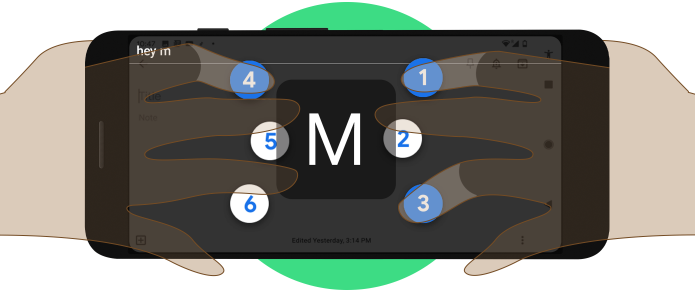
\includegraphics[width=10cm,height=10cm,keepaspectratio]{Figures/braille_keyboard.png}
    \caption{The 6 dot braille keyboard layout on an Android device is virtually identical to the iPhone equivalent, with dot 5 and 2 intentionally offset to make it as comfortable for users as possible \cite{braille}.}
    \label{fig:Jellybean}
\end{figure}

%----------------------------------------------------------------------------------------
%	SECTION 4
%----------------------------------------------------------------------------------------
\section{Hardware Accessibility}

Hardware accessibility in the realm of universal design is an area that will see much focus in this thesis. %%again to meta?
The following section reviews advancements made in the video game industry regarding designing for accessibility.

%-----------------------------------
%	SUBSECTION 1
%-----------------------------------
\subsection{Accessible Game Controller}

Microsoft's Xbox Adaptive Controller \cite{adaptive}, is a gaming controller that was designed in collaboration with multiple US associations and gamers with a disability, with accessibility in full focus.
This controller is designed with a large array of nineteen 3.5mm jacks and two USB 2.0 ports for external inputs \cite{adaptive} to allow a large degree of customisation for users with disabilities, so that they can plug in any digital switch input to suit their needs.
It is also in the affordable price range at AU\$130 \cite{accessiblecontroller} at the time of writing, compared to a 'standard' wireless controller which retails at AU\$90 \cite{standardcontroller} on Microsoft's online store.

\begin{figure} [h]
    \centering
    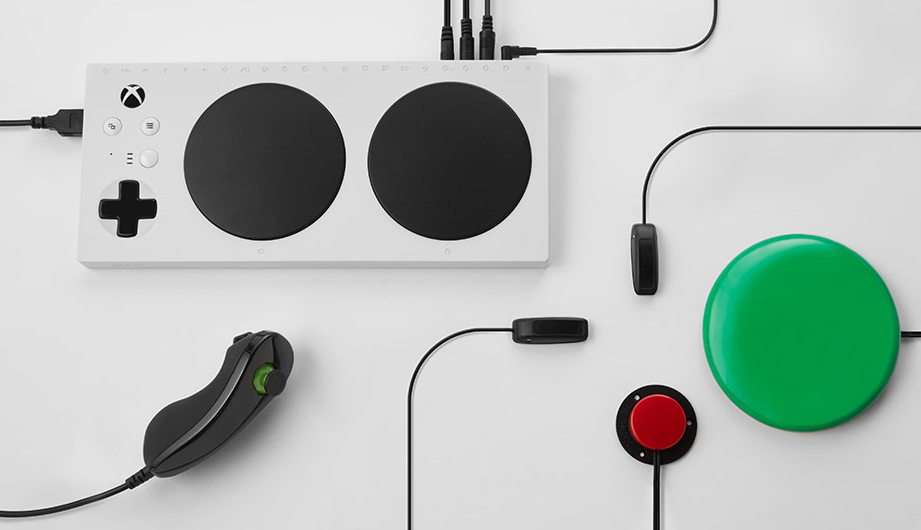
\includegraphics[width=10cm,height=10cm,keepaspectratio]{Figures/accessible_controller.png}
    \caption{Microsoft's accessible controller \cite{adaptive}, with a few examples of the types of switches that can be used to make playing video games significantly easier for those with a disability.}
    \label{fig:Jellybean}
\end{figure}

The Xbox Adaptive Controller is the first commercially available truly accessible controller, however, is not the first instance of this, as an earlier prototype revealed in 2011, called the Adroit Switchblade \cite{ablegamer}, in many ways set the groundwork in a partnership that lead to Microsoft's adaptation.
In an article interviewing Bryce Johnson, lead inclusive designer for Microsoft, Johnson states that "our standard controller has been optimised over the years around a primary use case – two thumbs and two index fingers” \cite{disabilitygaming}, a statement that he goes on to say has placed a barrier against playing for some people.
It is also evident that Microsoft has seen that the demographic of people with a disability is an otherwise untapped market.
While Microsoft's biggest video game console competitor, Sony has added software features to make their consoles more accessible \cite{sony}, neither Sony, nor Nintendo has yet to introduce an accessible controller with this level of usability and customisation.
% An article by Grammenos and others 

%----------------------------------------------------------------------------------------
%	SECTION 5
%----------------------------------------------------------------------------------------

\section{Digital Sovereignty and Right to Repair}

The 'Right to Repair' mantra falls under the Digital Sovereignty movement, where the focus is on how products can be designed to be transparent to the user and fully repairable by them [SOURCE?].
This is a concept that has recently seen more attention with electronics in the light of a trend where manufacturers are making it increasingly difficult for individuals to repair their own devices.
Electronic products such as smartphones are being designed with a limited lifespan under a concept that a paper by Bulow \cite{obsolescence} refers to as 'Planned Obsolescence', to encourage repeat purchases from customers in order to maximise profits.
Bulow goes on to also state that monopolists have an incentive to produce products with less durability as this takes away from the cost of developing a higher quality product.

On top of this, an article from Waldman shows that monopolists also have a high incentive to introduce a new electronic device with new stylistic changes, which in turn makes the preceding device obsolete \cite{obsolescence2}.
Waldman at the time, noted that technology company IBM, had changed their operating system in new computers which would no longer be compatible with older products, once again, an example of planned obsolescence.
Apple's iPhone, among other competitors, is a clear example of planned obsolescence at work today, with the consumer culture very much in favour of having with the 'latest and greatest' smartphone in their hand.
While it is important to note that consumer electronics are constantly innovating and therefore evolving, the distinction, in this case, is that manufacturers are not making their products 'upgradeable', which contributes to the shorter lifespan of the product.

%-----------------------------------
%	SUBSECTION 1
%-----------------------------------
\subsection{MEGAphone}

Digitally sovereign devices are becoming increasingly rare due to multiple factors such as increasing software and hardware complexity and protection of trade secrets.
The MEGAphone device is an initiative that aims to reclaim this dying concept, by introducing a mobile device that gives users full control over their data.
The appeal of the MEGAphone device is that it is intended as a platform in which users can modify and repair as they desire, and is therefore completely against planned obsolescence.

\begin{figure} [h]
    \centering
    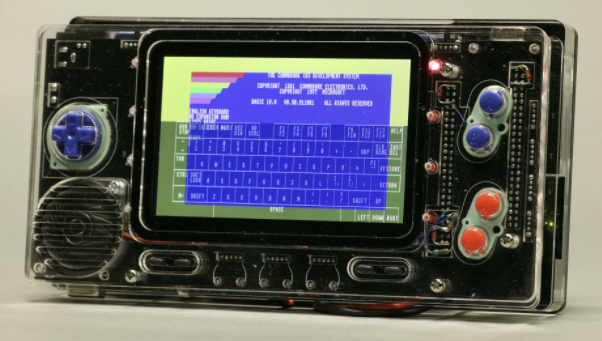
\includegraphics[width=10cm,height=10cm,keepaspectratio]{Figures/megaphone_concept.png}
    \caption{The first portable prototype of the MEGAphone device \cite{mega65}.}
    \label{fig:MEGAphoneConcept}
\end{figure}

In a CCC (Chaos Communication Camp) talk, Gardner-Stephen explains that their approach is to "start obsolete" so that they can't "get obsolete" and reduce the complexity of features to make it as accessible to individuals as possible \cite{mobilehistory}.
While this can be considered a niche approach, as true Digital Sovereignty is often sacrificed for many reasons such as the high complexity of modern operating systems (OS), Gardner-Stephen goes on to state that the Commodore 64 OS among others proved that simple architecture can still achieve a great deal.
This is all achieved with a relatively unique approach of implementing an FPGA as the heart of the device, thereby 

%-----------------------------------
%	SUBSECTION 2
%-----------------------------------
\subsection{Precursor}

'Precursor' is a pocketable, open-hardware mobile device with the same intention as the MEGAphone device; to provide users with a platform that they can trust, because they can audit all aspects of the device \cite{precursor}.
Unlike typical mobile devices, this project is intended as a development kit and is, therefore, more appealing to software developers looking for an open-source platform to test their code.

\begin{figure} [h]
    \centering
    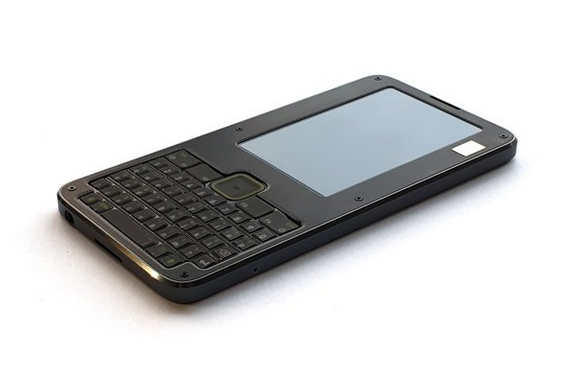
\includegraphics[width=10cm,height=10cm,keepaspectratio]{Figures/precursor.png}
    \caption{The Precursor mobile device is a crowd-funded project \cite{precursor}, seeking to put complete control in the hands of the user.}
    \label{fig:Precursor}
\end{figure}

Much like the MEGAphone device, Precursor is powered by a low power FPGA which compared to conventional CPUs, is remarkably efficient and allows for a far greater degree of freedom as they can quite literally redesign the architecture of the processor to suit their needs.
While FPGAs are currently far less powerful than CPUs in the same space, an article by Asano and others \cite{fpga} found that the Xilinx XC4VLX160 FPGA performed particularly well in image processing compared to an Intel CPU with four threads, four cores and a Geforce GTX280 GPU.
They noted that the limiting factor of an FPGA is its size and memory bandwidth, however, the 'fine-grained' parallelism of the FPGA showed that when dealing with a large number of parallel tasks (calculating two-dimensional filters in this instance), it became closer in performance to the GPU and more efficient than the CPU.
Given that CPUs are not particularly designed for large quantities of parallel tasks, this is somewhat expected, however, while GPUs are more effective at this use case, Asano and others observed that very small local memory within the GPU resulted in less efficient computations when dealing with more parallel instructions.
FPGAs have already shown that they can be effective and that will only improve with time.
The MEGAphone, much like the Precursor, has already proved that an FPGA can be a suitable choice for those not strictly looking for speed, but rather more freedom in how they develop their projects.

%----------------------------------------------------------------------------------------
%	SECTION 6
%----------------------------------------------------------------------------------------

\section{Effects of COVID-19} %% FIX THIS!!
%% discuss issues with supply in Australia due to COVID, need independence from imports
The recent global outbreak of the COVID-19 virus has threatened the DS movement and otherwise the 'Right to Repair' due to Australia's international trade dependence, particularly with China [SOURCE?].

%-----------------------------------
%	SUBSECTION 1
%-----------------------------------
\subsection{Capability Maintenance}

Capability Maintenance is a concept that looks at how the capabilities of products can be maintained, which is especially important in events that may trigger disruption of said capabilities.
A recent paper by Gardner-Stephen and Nabben \cite{capability} examines how key infrastructure can be maintained during global disruptions such as the COVID-19 pandemic.
In their findings, they note that there are very few projects working to address the challenges that capability maintenance provides.
Gardner-Stephen and Nabben suspect that the reason for this can be linked back to the concept of planned obsolescence, as the manufacturer stands to gain more by selling products that have a shorter lifespan \cite{obsolescence2}.

Capability Maintenance is relevant to the MEGAphone concept as it falls under the umbrella of DS.
Often people with a disability are the first to lose out on the accessibility of their devices as planned obsolescence introduces new software that no longer works with previous versions \cite{obsolescence2}. % revise this

%----------------------------------------------------------------------------------------
%	SECTION 7
%----------------------------------------------------------------------------------------

\section{Summary}
This chapter provides context for the proceeding chapters, as it establishes the criteria of the seven design principles, provides a distinction between 
Examples of UD and DS in practice are reviewed to further support the literature, in the form of accessible hardware, software and devices that look to promote keeping sensitive user data in the hands of the owner.
Capability Maintenance...
%% back up sources with more sources, always good to support